\section{Theoretischer Hintergrund}




\subsection{Freiheitsgrad}
"Der Freiheitsgrad $f$ eines Körpers ist die Anzahl der möglichen unabhängigen Bewegungen eines starren Körpers gegenüber einem Bezugskoordinatensystem"
\doublecite[35]{weber-Industrieroboter}.
Dabei ist $f$ die kleineste Menge von Parametern, die benötigt wird um die Lage des Körpers im Raum zu beschreiben
\doublecite[35]{weber-Industrieroboter}.
Abbildung \ref{fig:DOF_explanation} zeigt jeweils einen Quader mit dem Freiheitsgrad 3 und dem Freiheitsgrad 6.

\vspace{1em}

    \begin{figure}[H]
        \centering
        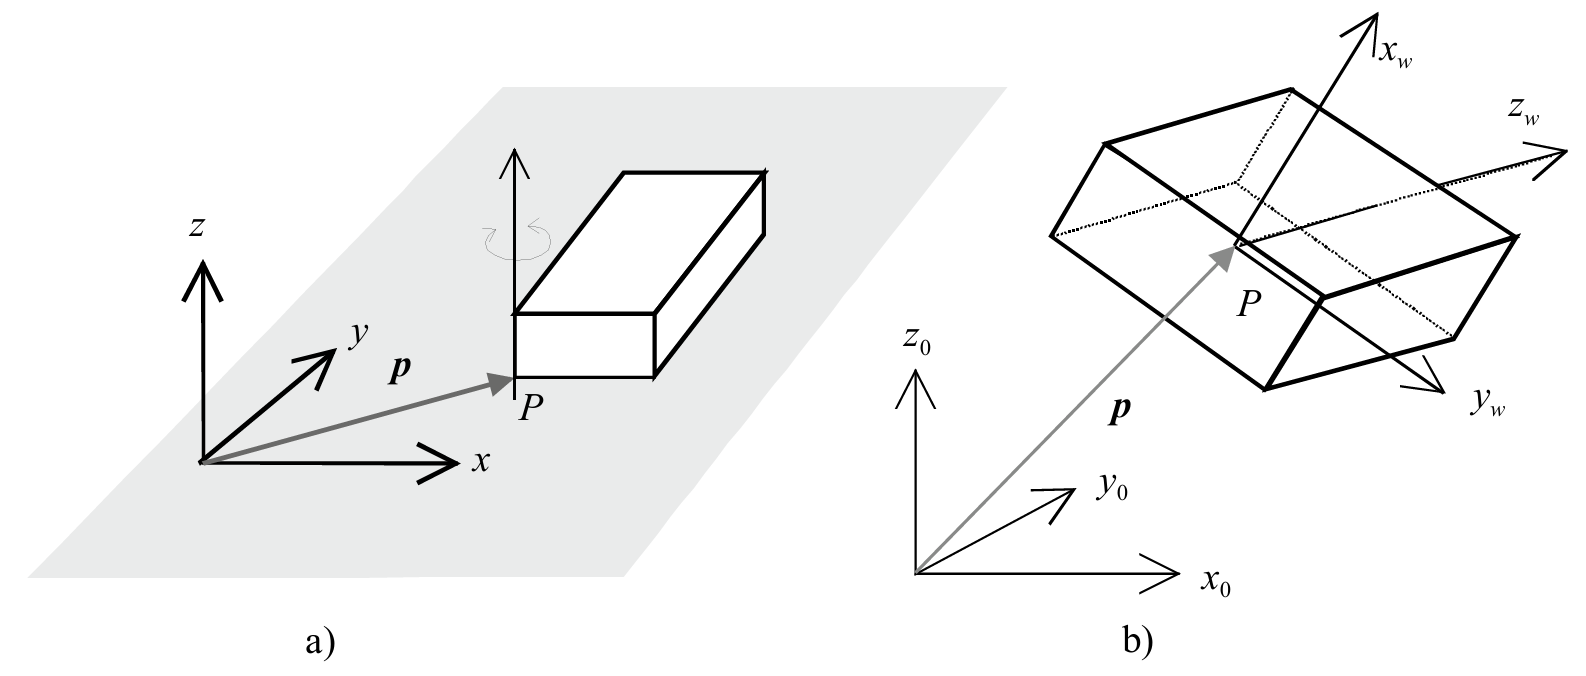
\includegraphics[width=1.0\textwidth]{images/DOF_exp.PNG}
        \caption{a) Quader mit Freiheitsgrad 3. b) Quader mit Freiheitsgrad 6. Quelle: \doublecite[35]{weber-Industrieroboter}}
        \label{fig:DOF_explanation}
    \end{figure}

\vspace{1em}

Der Quader in Abbildung \ref{fig:DOF_explanation} a) hat den Freiheitsgrad 3 und kann nur auf einer Ebene bewegt werden die durch den grauen Bereich dargestellt wird.
Die Position des Quaders wird durch einen Ortsvektor eindeutig beschrieben.
Zusätzlich kann der Quader noch um eine Achse gedreht werden die Senkrecht zur Ebene steht und durch den Punkt $P$ geht.
Anhand des Ortsvektors und des Drehwinkels wird die Lage des Quaders auf der Ebene eindeutig beschrieben.

Der Quader in Abbildung \ref{fig:DOF_explanation} b) hat den Freiheitsgrad 6 und kann sich frei im Raum bewegen.
Die Position eines Punktes $P$, für den sich der Schwerpunkt des Quaders eignet, wird durch einen Ortsvektor mit 3 Komponenten beschrieben.
Das sind die 3 Freiheitsgrade der Translation. Hinzu kommen die 3 Freiheitsgrade der Rotation, da der Quader frei um 3 Achsen im Raum rotieren kann
\doublecite[35]{weber-Industrieroboter}.

In der Robotik bezeichnet der Arbeitsraum den Bereich im Raum, welcher vom Roboter erreicht werden kann.
Ein Roboter der sich im Euklidischen Raum bewegt hätte den Arbeitsraum $T \subset \mathbb{R}^3 \times SO(3)$

Neben dem eben erwähnten Freiheitsgrad der sich auf den Arbeitsraum bezieht gibt es noch den Freiheitsgrad im Konfigurationsraum.
In der Mechanik bezeichnet man die kleinste Menge von Parametern, die benötigt werden um die Lage eines Systems im Arbeitsraum zu beschreiben als Konfiguration eines Systems, die durch einen Punkt $q$ dargestellt werden kann.
Die Menge aller möglichen Konfigurationen bildet den sogenannten Konfigurationsraum (c-space) $C$, sodass $q \in C$.
Ein Roboter mit 2 Drehgelenken hätte beispielsweise den Konfigurationsraum $C \subset SO(1) \times SO(1)$ und seine Konfiguration könnte anhand von zwei Parametern $(q_1,q_2)$ beschrieben werden.
Folglich hätte dieser Roboter einen Freiheitsgrad von 2 im Konfigurationsraum.

Jeder Punkt im Konfigurationsraum kann auf einen Punkt im Arbeitsraum abgebildet werden, wobei i.A nicht jeder Punkt im Arbeitsraum auf einen Punkt im Konfigurationsraum abgebildet werden kann.
\doublecite[78]{Robotics_Vision_and_Control}.



\subsection{Industrieroboter}
Ein Industrieroboter (engl. industrial-robot, manipulator), ist gemäß DIN EN ISO 10 218-1 ein frei Programmierbarer Mehrzweck-Manipulator,
der in 3 oder mehr Achsen Programmierbar ist
\doublecite[17]{Industrieroboter}.
Er ist universell einsetzbar, und wird häufig für Schweiß-, -Lackierarbeiten, Montageaufgaben und viele weitere Fertigungs- und Handhabeaufgaben verwendet
\doublecite[2-3]{weber-Industrieroboter}.
Obwohl ein Industrieroboter sich, im Gegensatz zu mobilen Robotern, nicht frei durch den Raum bewegen kann,
kann er statt an festen Orten auch beweglich angeordnet werden
\doublecite[17]{Industrieroboter}.
Typischerweise besteht ein solcher Roboter aus mehreren starren Segmenten, sogenannten Gliedern (engl. links), welche durch Gelenke bzw. Achsen (engl. joints)
miteinander verbunden sind. Der Industrieroboter führt seine Bewegung über seine Gelenke und Glieder aus, wobei ihre Anordnung die kinematische Struktur des Roboters bestimmt.
Es gibt zwei Hauptklassen kinematischer Strukturen:
Die serielle Kinematik und die Parallelkinematik. Die Parallelkinematik wird nur in spezielleren Fällen verwendet wo eine besonders schnelle Handhabung notwendig ist
und wird in dieser Arbeit nicht näher beleuchtet.
Die serielle Kinematik ist in der Industrie häufiger verteten.
Die folgende Abbildung zeigt einen Industrieroboter von KUKA, welcher 6 Drehgelenke hat und zu den Seriellen Robotern gehört.

 \vspace{1em}

    \begin{figure}[H]
        \centering
        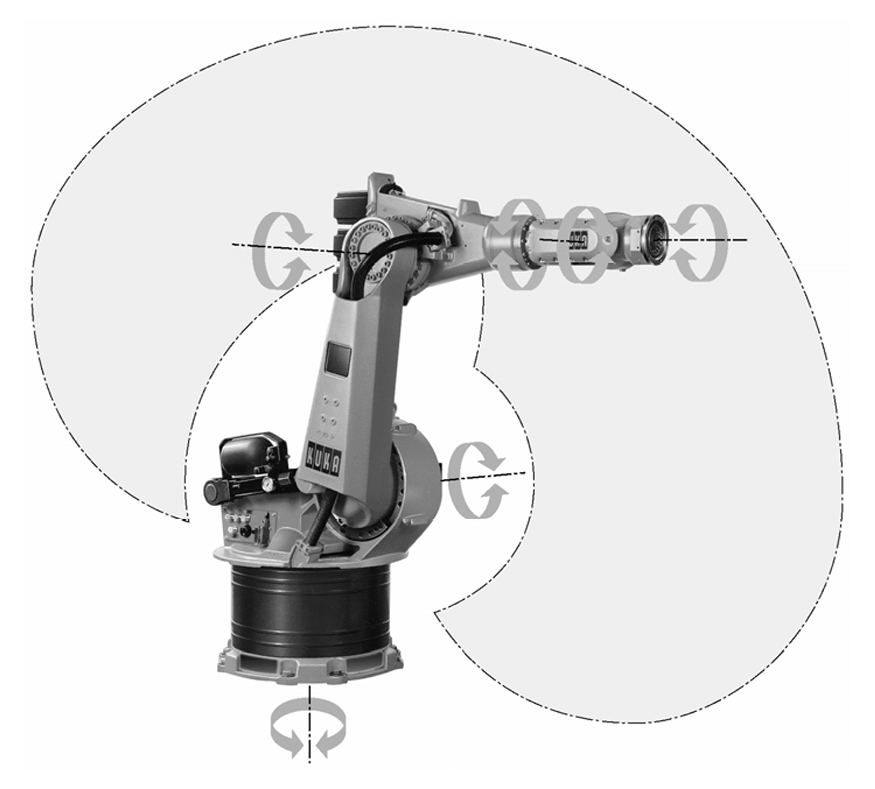
\includegraphics[width=0.5\textwidth]{images/kuka-ir.PNG}
        \caption{Industrieroboter von Kuka. Quelle: \doublecite[6]{weber-Industrieroboter}}
        \label{fig:KUKA-IR}
    \end{figure}

\vspace{1em}


Die durch Pfeile markierten Elemente des Roboters sind die Drehgelenke.
Durch Drehung dieser Gelenke werden die damit verbundenen Glieder im Raum bewegt.
Die Glieder stehen aneinandergereiht zueinander und bilden eine kinematische Kette, was das Merkmal für Roboter mit serieller Kinematik ist
\doublecite[3-6]{weber-Industrieroboter}.
Am oberen Ende des Roboters befindet sich ein Flansch, an den ein beliebiges Werkzeug, wie beispielsweise ein Greifer angebracht werden kann
\doublecite[17]{Industrieroboter}.
Ein solches Werkzeug wird dann als Endeffektor bezeichnet und kann als letztes Glied aufgefasst werden.
Die Werkzeugspitze des Endeffektors wird als Tool Center Point (TCP) bezeichnet und wird verwendet um die sogenannte Pose (Position und Orientierung) des Endeffektors, im Raum zu beschreiben.
Die Aufgabe eines jeden Industrieroboters ist es den Endeffektor geeignet im Raum zu bewegen um eine bestimmte Tätigkeit auszuführen.
Dies wird durch eine passende Konfiguration der Achsen erreicht.
Die Bewegungsmöglichkeit des Roboters hängt direkt von der Anzahl der Achsen ab.
Man spricht bei der Anzahl unabhängig angetriebener Achsen vom mechanischen- oder Getriebe-Freiheitsgrad.
Bei mindestens 6 unabhängig angetriebener Achsen in geeigneter Anordnung hat der Endeffektor den Freiheitsgrad 6 und kann eine beliebige Pose einnehmen
\doublecite[3-6]{weber-Industrieroboter}.
Der Bereich im Raum, der vom Endeffektor erreicht werden kann, wird Arbeitsraum des Roboters genannt und ist abhängig von der Bewegunsform,
der Anordnung und Anzahl der Achsen sowie der Länge der einzelnen Glieder.
Der Arbeitsraum eines Industrieroboters kann z.B quaderförmig, zylindrisch oder Kugelförmig sein.
der Arbeitsraum eines klassichen Sechs-Achs-Knickarmroboters ist kugelförmig wie in Abbildung \ref{fig:KUKA-IR} durch den grauen Bereich dargestellt ist.
\doublecite[18]{Industrieroboter}.
Es gibt auch Roboter mit mehr Achsen und einem höheren Freiheitsgrad, sowie weniger Achsen und einem geringeren Freiheitsgrad.
Die Kinematik bei Robotern mit einem Freiheitsgrad $>$ 6 ist redundant und gilt als überbestimmt
\doublecite[4-5]{weber-Industrieroboter}.
Abbildung \ref{fig:lbr} zeigt den Leichtbauroboter iiwa von KUKA mit 7 Drehachsen.

\vspace{1em}

    \begin{figure}[H]
        \centering
        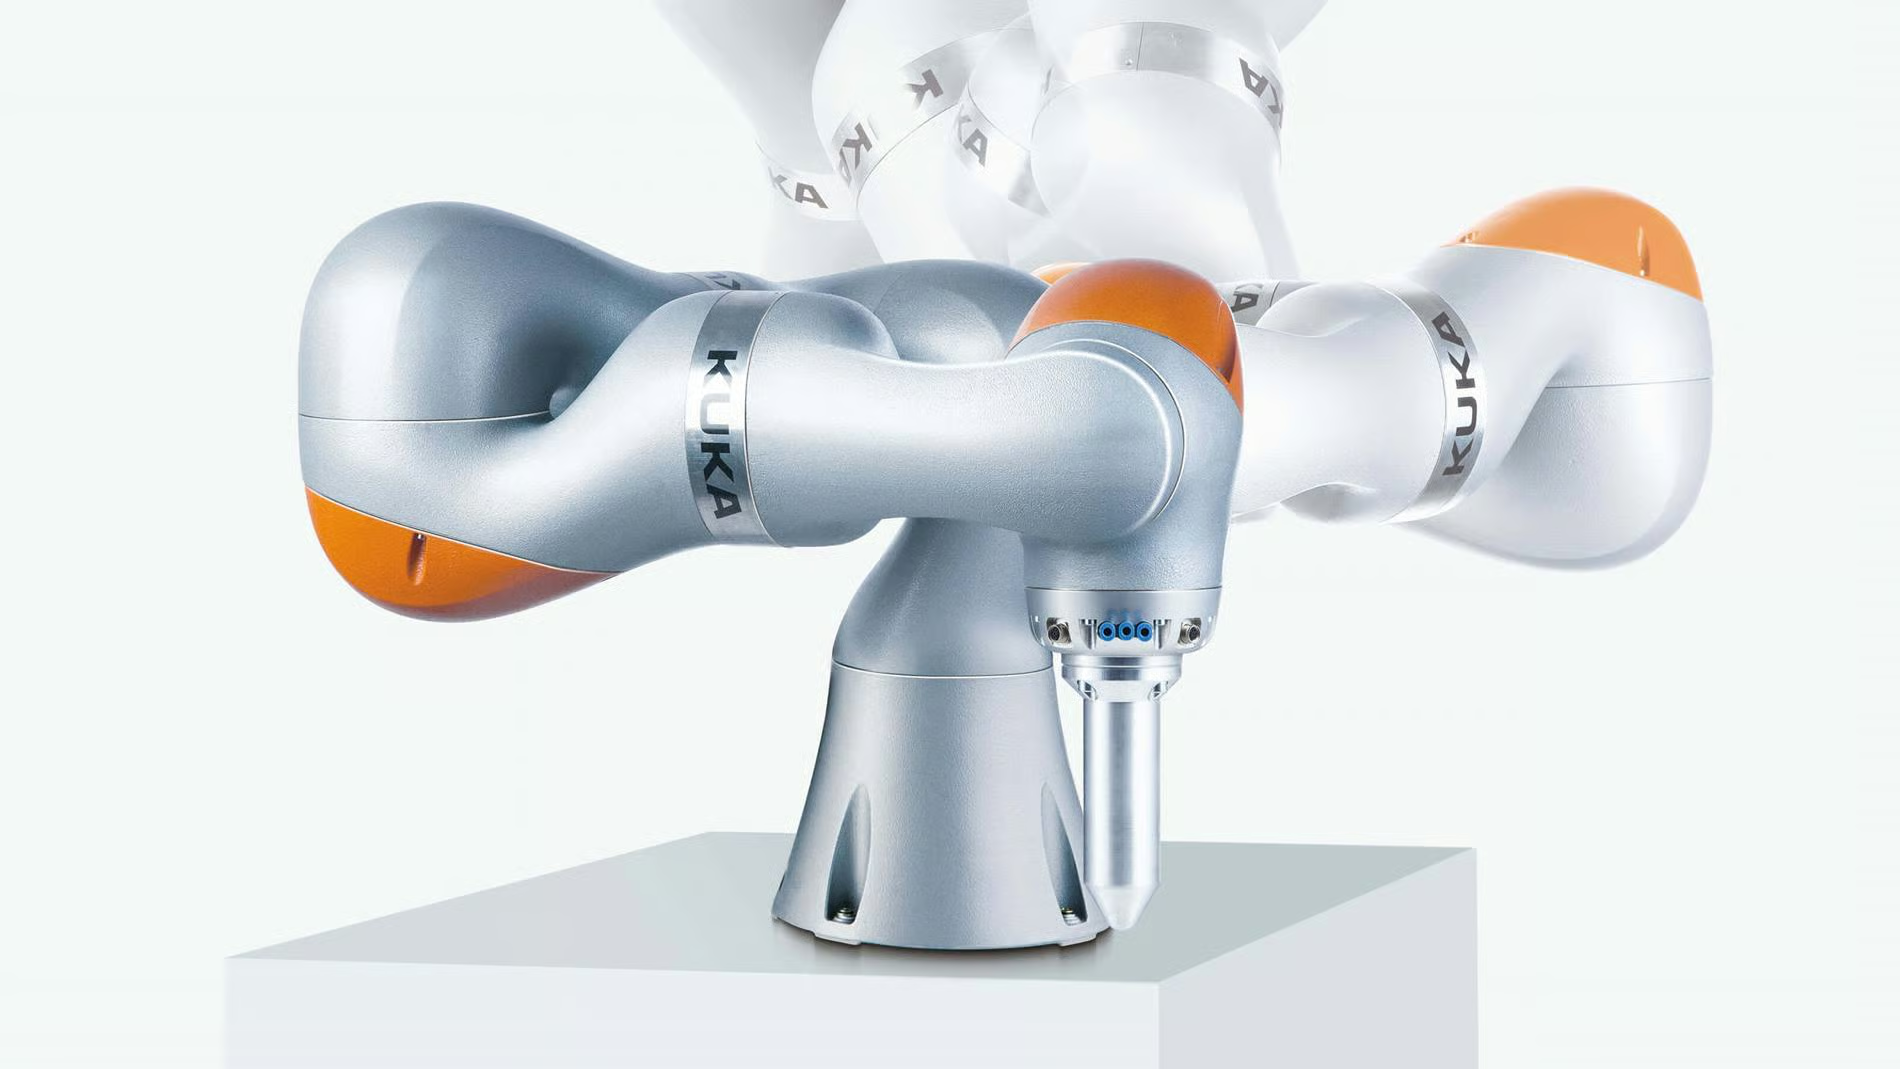
\includegraphics[width=1.0\textwidth]{images/lbr2.png}
        \caption{Leichtbauroboter iiwa von KUKA. Quelle: \doublecite[]{lbr_image}}
        \label{fig:lbr}
    \end{figure}

\vspace{1em}



Der Vorteil der überbestimmten Kinematik liegt darin, dass die Feinbewegung des Endeffektors verbessert wird und dieser besser mit bewegenden Objekten synchronisiert werden kann.
Darüber hinaus sind Roboter mit 7 Drehachsen in zusammenarbeit mit Menschen zu bevorzugen,
da sie Hindernisse besser umfahren und sich somit der Bewegung von Menschen besser anpassen können
\doublecite[]{WEINGARTSHOFER2019507}.

Damit ein Industrieroboter durch Bewegung eine spezifische Tätigkeit ausführen kann, muss er zunächst programmiert werden.
Dabei "[...] wird in der Robotik zwischen zwei wesentlichen Verfahrensgruppen unterschieden: Online- und Offline-\-Pro\-grammie\-rung" \doublecite[149]{Industrieroboter}.
Die Online-Programmierung wird meistens durch sogenannte Teach-In verfahren durchgeführt. Dabei steuert eine Person den Roboter mithilfe eines Programmierhandgeräts
an bestimmte Punkte im Raum. Anschließend wird diese Position gespeichert, sodass sie in Zukunft ohne erneute Steuerung angefahren werden kann.
Die Offline-Programmierung umfasst die Verfahren zur Programmierung des Roboters ohne diesen einzubinden und eignet sich besonders wenn der Roboter komplexe Bahnen verfahren muss
\doublecite[149-150]{Industrieroboter}.
Dabei stellt die textuelle Programmierung, bei der die "[...] Befehle in eine Textdatei geschrieben werden und [...] sequentiell von der Robotersteuerung abgeabeitet [...]" werden,
das am häufigsten verwendete Verfahren dar
\doublecite[149]{Industrieroboter}. 

In der heutigen Zeit findet die simulationsgestützte Programmierung, welche ebenfalls zu den Offline-Verfahren gehört, immer mehr Anwendung.     %nachfragen ob das noch als sinngemäß übernommen gilt
Schon innerhalb des Produktionsprozesses sämtlicher Roboter-Komponenten werden CAD-Daten erstellt, die ein Digitales Modell dieser Komponenten darstellen.
Mithilfe dieser CAD-Daten kann innerhalb von simulationsgestützten Offline-Tools ein Roboter dargestellt und simuliert werden.
Diese Art der Roboter-Programmierung birgt viele Vorteile wie das Testen auf Kollision ohne Gefahr oder die Zeit und Kostenberechnung des Robotereinsatzes in der Planungsphase.
Mit der Erstellung dieser simulationsgestützten Offline-Tools geht allerdings ein hohes Expertenwissen im bereich der Robotik einher
\doublecite[150-152]{Industrieroboter}. 



\subsection{Vorwärtstransformation}
Die Vorwärtstransformation, auch direktes Kinematisches Problem genannt, ist ein zentrales Konzept für die Steuerung und Simulation von Industrierobotern.
Sie ist eine eindeutige Abbildung von Gelenkkoordinaten im Konfigurationsraum auf kartesische Koordinaten im Arbeitsraum.
Die Pose des Roboters im Arbeitsraum wird vollständig durch die Gelenkkoordinaten beschrieben.
Insbesondere ist dann auch die Pose des Endeffektors eindeutig festgelegt.
Die folgende Abbildung zeigt den schematischen Ablauf der Vorwärtstransformation.

\vspace{1em}

    \begin{figure}[H]
        \centering
        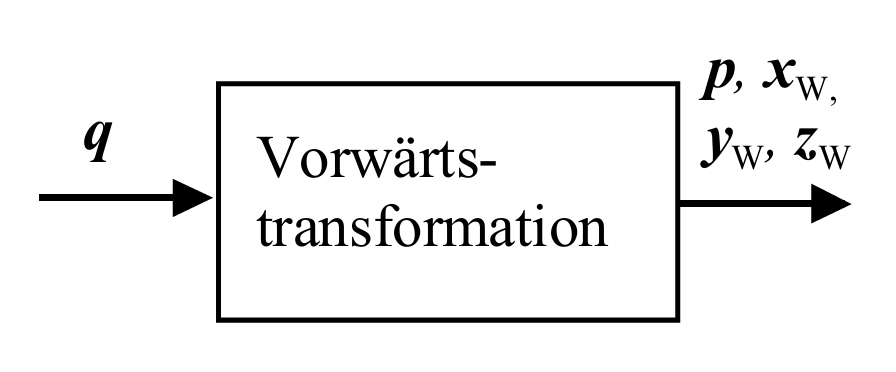
\includegraphics[width=0.5\textwidth]{images/forward_kin.PNG}
        \caption{schematischer Aufbau der Vorwärtstransformation. Quelle: \doublecite[49]{weber-Industrieroboter}}
        \label{fig:forward_kinematic}
    \end{figure}

\vspace{1em}

Sei $q$ ein Tupel mit $q = (q_1,q_2,....,q_n)^T$, welches die Ge\-lenk\-koordinaten enthält.
Der Ortsvektor $p$, ausgehend vom Ursprung des Bezugskoordinatensystems und die Orientierung, beschrieben durch die Basisvektoren $x_W,y_W,z_W$ beschreiben die Pose des Endeffektors.
Durch die Vor\-wärts\-trans\-for\-ma\-tion können diese aus dem Tupel $q$ berechnet werden.
Genauer betrachtet ist die Vorwärtstransformation die Multiplikation mehrerer Homogener Transformationsmatrizen, die jeweils die Lage eines einzelnen Gelenks im Bezug auf das vorherige Gelenk beschreiben.
\[
T_W(q) = \prescript{n}{0}{T}(q) = \prescript{1}{0}{T}(q_1) \cdot \prescript{2}{1}{T}(q_2)\cdot\cdot\cdot\prescript{n-1}{n-2}{T}(q_{n-1}) \cdot \prescript{n}{n-1}{T}(q_n)
\]
Für die Berechnung der Homogenen Transformationsmatrizen wird in der Robotik die sogenannten Denavit-Hartenberg-Notation verwendet, aus der dann die Denavit-Hartenberg-Matrizen resultieren.
\doublecite[49-50]{weber-Industrieroboter}.




\subsection{Denavit-Hartenberg-Konvention}
Die Denavit-Hartenberg-Konvention wurde 1955 von Jacques Denavit und Richard Hartenberg eingeführt und ist ein weit verbreitetes Werkzeuge zur Beschreibung der Pose eines Roboters im Raum.
Sie ist ein standardisiertes Verfahren zur Modellierung der Kinematik serieller Roboter.
Ziel der Konvention ist es, die Position und Orientierung jedes Gliedes relativ zum vorhergehenden Glied mit einem minimalen Satz von Parametern darzustellen.
Die Transformation von einem Glied zum nächsten wird durch eine homogene Transformationsmatrix beschrieben, die vier aufeinanderfolgende Operationen zusammenfasst:
zwei Rotationen und zwei Translationen.
Daraus ergeben sich die vier Denavit-Hartenberg-Parameter(DH-Parameter):

  $\theta_i$: der Gelenkwinkel, Rotation um die z-Achse

  $d_i$: Verschiebung entland der z-Achse

  $a_i$: Verschiebung entlang der x-Achse

  $\alpha_i$: Rotation um die x-Achse
\\\\ 
Mit diesen Parametern lässt sich für jedes Glied eine Homogene Transformationsmatrix aufstellen die fest mit dem Glied verbunden ist und die Position und Orientierung in Bezug zum vorherigen Koordinatensystem beschreibt.
Die folgende Abbildung zeigt eine schematische Zeichnung eines Knickarmroboters mit 6 Gelenken und entsprechenden Denavit-Hartenberg-Koordinatensystemen.

\vspace{1em}

    \begin{figure}[H]
        \centering
        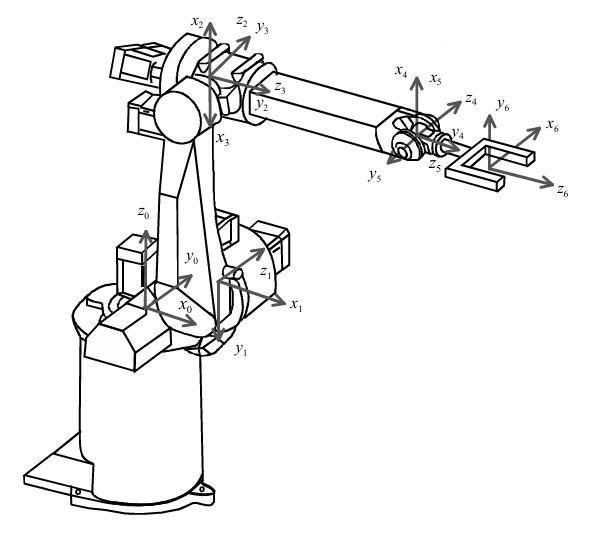
\includegraphics[width=0.5\textwidth]{images/DH_explain2.PNG}
        \caption{schematische Zeichnung eines Knickarmroboters mit 6 Gelenken und DH-Koordinatensystemen. Quelle: \doublecite[39]{weber-Industrieroboter}}
        \label{fig:DH_explanation}
    \end{figure}

\vspace{1em}

Die erste Transformationsmatrix beschreibt das Basiskoordinatensystem $K_0$ und ist fest mit der ruhenden Basis, also dem ersten Glied verbunden.
Der Ursprung von $K_0$ muss dabei auf die erste Gelenkachse gelegt werden.
Die $z_0$-Achse von $K_0$ zeigt entlang der ersten Gelenkachse.
Die $x_0$- und $y_0$-Achse sind anschließend frei wählbar unter der bedingung das die zugehörigen Einheitsvektoren $x_0, y_0$ und $z_0$ ein Rechtssystem bilden.

Jedes weitere Koordinatensystem $K_i$,
welches durch eine Transformationsmatrix repräsentiert wird, das aus den DH-Parametern gebildet wird, muss einen Satz fest definierter Bedingungen erfüllen:
Der Ursprung von $K_i$ sollte auf der Gelenkachse $i+1$ liegen.
Wenn sich die Gelenkachsen $i$ und $i+1$ schneiden, muss der Ursprung von $K_i$ im Schnittpunkt dieser beiden Achsen liegen.
Verlaufen die beiden Achsen jedoch parallel, kann der Ursprung von $K_i$ beliebig auf die Gelenkachse $i+1$ gelegt werden.
Wenn die Achsen sich nicht schneiden und auch nicht parallel sind wird die gemeinsame Normale der Gelenkachse $i$ und $i+1$ berechnet und der Ursprung von $K_i$ auf den
Schnittpunkt der gemeinsamen Normalen mit der Gelenkachse $i+1$ gelegt.

Die Gesamttransformation vom Basis-Koordinatensystem $K_0$ zum Koordinatensystem des Endeffektors $K_i$ ergibt sich durch sukzessive Multiplikation aller einzelnen Transformationsmatrizen $K_0, K_1, ..., K_n$ entlang der kinematischen Kette.
Das entspricht der durchführung der Vorwärtstransformation.
\doublecite[38-44]{weber-Industrieroboter}




\subsection{Rückwärtstransformation}
Die Rückwärtstransformation, auch als inverse Kinematik bezeichnet, wird verwendet um aus der gegebenen Pose des Endeffektors die Gelenkkoordinaten $q_0,q_1...,q_n$ zu berechnen
und stellt somit das gegenstück zu Vorwärtstransformation dar.
Im Gegensatz zur Vorwärtstransformation bringt die Rückwärtstransformation einige Schwierigkeiten wie Mehrdeutigkeiten und Singularitäten mit sich.
Eine Pose des Endeffektor innerhalb des Arbeitsraums kann unter umständen mit mehreren verschiedenen Gelenkstellungen des Roboters erreicht werden.
Die folgende Abbildung veranschaulicht eben diesen Umstand.


\vspace{1em}

    \begin{figure}[H]
        \centering
        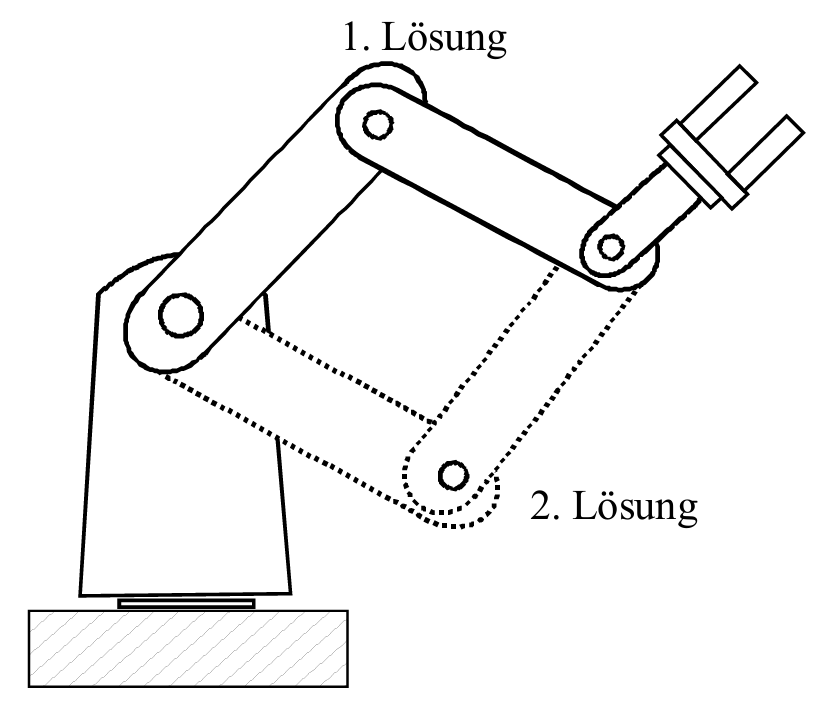
\includegraphics[width=0.5\textwidth]{images/ik_planar_exp.PNG}
        \caption{schematische Zeichnung eines Planarroboters mit 2 Achsen. Quelle: \doublecite[51]{weber-Industrieroboter}}
        \label{fig:ik_planar_explanation}
    \end{figure}

\vspace{1em}




Unendlich viele Lösungen gibt es z.B dann, wenn der Roboter eine Position einnimmt, in der er einen Freiheitsgrad verliert und dadurch gleiche Änderungen an bestimmten Gelenken 
zu gleichen Änderungen am Endeffektor führen. Die folgende Abbildung veranschaulicht das Auftreten einer solchen Singularität.

\vspace{1em}

    \begin{figure}[H]
        \centering
        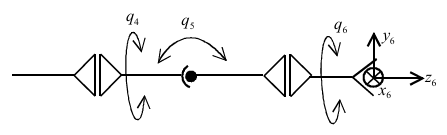
\includegraphics[width=0.5\textwidth]{images/ik_singularity_explain.PNG}
        \caption{schematische Zeichnung einer Gelenkstellung die zu Unendlich vielen Lösungen führt. Quelle: \doublecite[51]{weber-Industrieroboter}}
        \label{fig:ik_singularity_explain}
    \end{figure}

\vspace{1em}

In der vorliegenden Gelenkstellung von $q_5$ gibt es zu jeder Gelenkstellung von $q_4$ eine Gelenkstellung von $q_6$ die den Endeffektor in der gegebenen Pose beschreibt.
Daraus folgen unendlich viele Konfigurationen die für den Roboter möglich wären um die gegebene Pose des Endeffektors zu erreichen.
Um solche Singularitäten aufzulösen kann ein Gütekriterium als Nebenbedingung formuliert werden, um eine definierte Lösung zu erhalten.

Für die gängigen Knickarmroboter mit 6 Gelenken kann das geometrische verfahren angewendet werden um aus der Endeffektor Pose die Gelenkkoordinaten zu erhalten.
Diese Methode wird in der Praxis bevorzugt angewendet. 
Für viele andere Roboter, wie beispielsweise Knickarmroboter mit mehr als 6 Gelenken kann das geometrische Verfahren nicht angewendet werden.
In solchen Fällen werden Numerische Verfahren wie zum Beispiel das Newton-Raphson-Verfahren verwendet um eine geeignete Näherungslösung zu approximieren
\doublecite[49-56]{weber-Industrieroboter}.
Da in dieser Arbeit das numerische Verfahren mittels Newton-Raphson-Verfahren dem geometrischen Verfahren vorgezogen wurde, wird dieses in dieser Arbeit 
noch eine ausführlichere Rolle spielen.





\subsection{Unified Robot Description Format (URDF)}
URDF ist ein portables, XML-basiertes Dateiformat, welches den Austausch von Ro\-bo\-ter-\-Modellen erlaubt.
Es erleichtert das einbinden von Roboter-Modellen in Simulationssoftware und ist in der Robotik sehr verbreitet.
URDF-Dateien werden oft mit Xacro, einer XML macro Sprache erstellt um die Dateien kürzer und besser lesbar zu machen.
URDF-Dateien enthalten viele Informationen wie die Orientierung und Position von Gelenken und Gliedern, den Pfad zu den 3D-Modellen,
welche die Glieder repräsentieren, Hierarchien innerhalb der kinematischen Kette sowie Minimal- und Maximal-Grenze der Gelenke und viele weitere
Technische Informationen.
Es existieren viele URDF-Dateien zu bekannten Industrierobotern die aus dem Internet von Seiten wie Github frei Runtergeladen und verwendet werden können
\doublecite[270-271]{Robotics_Vision_and_Control}.

